\documentclass[a4paper,12pt]{article}
\usepackage{graphicx}
\usepackage{amsmath}
\usepackage{hyperref}
\usepackage{listings}
\usepackage{xcolor}
\documentclass{article}
\usepackage{longtable}
\usepackage{pgfplots}
\usepackage{pgfplotstable}
\pgfplotsset{compat=1.18}

\title{Análise de Algoritmos de Ordenação}
\author{Dante Ungarelli e Saulo Ferraz}
\date{\today}

\lstset{
    language=Python,
    basicstyle=\ttfamily\footnotesize,
    keywordstyle=\color{blue},
    commentstyle=\color{gray},
    stringstyle=\color{orange},
    showstringspaces=false,
    frame=single,
    breaklines=true
}

\begin{document}
\begin{figure}
    \centering
    \includegraphics[width=5cm]{image.png}
\end{figure}


\maketitle

\section{Introdução}
\subsection{Breve introdução sobre a importância da ordenação de dados.}
A ordenação de dados é uma operação fundamental em ciência da computação e desempenha um papel crucial em várias aplicações, como busca de informações, otimização de processos e análise de dados. Um conjunto de dados ordenado permite que outras operações, como pesquisa binária, sejam executadas de forma mais eficiente, melhorando o desempenho de sistemas computacionais. Além disso, muitos algoritmos complexos dependem de uma etapa inicial de ordenação para funcionarem corretamente. Devido à sua importância prática e teórica, o estudo de algoritmos de ordenação é uma área amplamente explorada, sendo essencial compreender o comportamento desses algoritmos em diferentes cenários, para tomar decisões informadas sobre qual abordagem é mais adequada em cada contexto.
\subsection{Objetivo do trabalho e algoritmos a serem analisados.}
O objetivo deste trabalho é realizar uma análise empírica de diferentes algoritmos de ordenação, comparando tanto seus aspectos teóricos quanto práticos. Essa análise permitirá explorar como os algoritmos se comportam em diferentes situações, medindo seu desempenho em termos de tempo de execução, número de comparações e número de trocas realizadas. Serão analisados os algoritmos Bubble Sort, Selection Sort, Insertion Sort, Merge Sort, Quick Sort e Heap Sort. A implementação desses algoritmos será testada em listas de tamanhos variados (1.000, 10.000, 50.000, 100.000 elementos), com diferentes tipos de distribuição de dados (ordenadas, inversamente ordenadas e aleatórias), de modo a identificar as vantagens e limitações de cada técnica de ordenação em cenários específicos.
\section{Revisão Teórica}
\subsection{Descrição teórica de cada algoritmo de ordenação.}
\subsubsection{Bubble Sort: Complexidade, in place, estabilidade.}
O Bubble Sort é um algoritmo de ordenação que percorre a lista repetidas vezes, comparando elementos adjacentes e trocando-os se estiverem fora de ordem. O processo se repete até que nenhum elemento precise ser trocado, indicando que a lista está ordenada. Sua complexidade de tempo no pior e no caso médio é \(O(n^2)\), e no melhor caso (quando a lista já está ordenada), é \(O(n)\). O Bubble Sort é um algoritmo \textit{in-place}, o que significa que ele não requer memória extra além da própria lista que está sendo ordenada. Além disso, é um algoritmo estável, ou seja, não altera a ordem relativa de elementos com valores iguais.
\subsubsection{Selection Sort: Complexidade, in place, estabilidade.}
O Selection Sort ordena a lista selecionando repetidamente o menor elemento da parte não ordenada e trocando-o com o primeiro elemento da parte não ordenada. Ele continua esse processo até que toda a lista esteja ordenada. A complexidade do Selection Sort é \(O(n^2)\) em todos os casos, pois ele percorre a lista inteira para encontrar o menor elemento, independentemente da ordenação inicial. O algoritmo é \textit{in-place}, já que realiza a ordenação diretamente na lista, sem uso de memória adicional significativa. No entanto, o Selection Sort não é estável, pois pode alterar a posição relativa de elementos iguais durante as trocas.
\subsubsection{Insertion Sort: Complexidade, in place, estabilidade.}
O Insertion Sort constrói a lista ordenada inserindo um elemento por vez na posição correta. Ele percorre a lista da esquerda para a direita, movendo os elementos à medida que encontra o local apropriado para o novo elemento. No melhor caso, quando a lista já está ordenada, sua complexidade é \(O(n)\), mas no caso médio e no pior caso, é \(O(n^2)\). O Insertion Sort é um algoritmo \textit{in-place}, pois ordena os elementos diretamente na lista sem exigir espaço adicional. Além disso, é estável, já que mantém a ordem relativa dos elementos iguais.
\subsubsection{Merge Sort: Complexidade, in place, estabilidade.}
O Merge Sort segue o paradigma de divisão e conquista, dividindo a lista em duas sublistas de tamanhos iguais até que cada sublista contenha apenas um elemento, e então combina essas sublistas de forma ordenada. A complexidade do Merge Sort é \(O(n \log n)\) tanto no melhor, no pior, quanto no caso médio, tornando-o mais eficiente do que os algoritmos quadráticos em grandes conjuntos de dados. No entanto, ele não é \textit{in-place}, pois requer espaço adicional para armazenar as sublistas temporárias. O Merge Sort é estável, pois preserva a ordem relativa de elementos iguais durante o processo de combinação.
\subsubsection{Quick Sort: Complexidade, in place, estabilidade.}
O Quick Sort também utiliza a abordagem de divisão e conquista, selecionando um pivô e particionando os elementos em torno desse pivô, de modo que os menores fiquem à esquerda e os maiores à direita. O processo é então repetido recursivamente nas sublistas resultantes. No caso médio e no melhor caso, sua complexidade é \(O(n \log n)\), mas no pior caso, que ocorre quando o pivô é mal escolhido, a complexidade pode ser \(O(n^2)\). O Quick Sort é \textit{in-place}, pois organiza os elementos dentro da lista original, mas não é estável, uma vez que a troca de elementos pode alterar a ordem relativa de elementos iguais.
\subsubsection{Heap Sort: Complexidade, in place, estabilidade.}
O Heap Sort baseia-se na estrutura de dados heap para ordenar a lista. Primeiro, ele constrói um heap máximo a partir da lista original, e em seguida, remove o maior elemento (a raiz do heap) e reorganiza o heap restante. Esse processo é repetido até que a lista esteja ordenada. A complexidade do Heap Sort é \(O(n \log n)\) em todos os casos. Ele é um algoritmo \textit{in-place}, já que realiza a ordenação na própria lista sem uso de memória adicional significativa. No entanto, o Heap Sort não é estável, uma vez que a estrutura do heap pode modificar a ordem relativa dos elementos iguais durante o processo de reordenação.

\section{Metodologia}
\subsection{Descrição do ambiente de teste (hardware e software).}
O hardware utilizado para realizar os testes foi um notebook modelo Acer Nitro 5 com as seguintes configurações:

\textbf{Processador}: Intel(R) Core(TM) i5-10300H CPU @ 2.50GHz   2.50 GHz

\textbf{Memoria RAM}: 24G DDR4

\textbf{Armazenamento}: 256GB SSD e 1TB HD

\textbf{Placa de vídeo}: NVIDIA GEFORCE GTX 1650

\textbf{SO}: Windowns 11 \\
O ambiente de teste utilizado para implementação dos algoritmos de ordenação foi o Visual Studio Code, versão 1.94.0 na linguagem Python, versão 3.11.3. Para medir o tempo de execução dos algoritmos, utilizou-se a biblioteca "time", e as listas aleatórias foram geradas utilizando a biblioteca "random".

\subsection{Implementação dos algoritmos (código).}
 \textbf{Bubble sort: } \\
\begin{lstlisting}[language=Python]
import time
import random

# Função para gerar listas de acordo com a distribuição escolhida
def gerar_lista(tamanho, tipo_distribuicao):
    if tipo_distribuicao == 1:
        return list(range(tamanho))
    elif tipo_distribuicao == 2:
        return list(range(tamanho, 0, -1))
    elif tipo_distribuicao == 3:
        return random.sample(range(tamanho), tamanho)

# Implementação do Bubble Sort 
def bubble_sort(arr):
    n = len(arr)
    comparacoes = 0
    trocas = 0
    for i in range(n):
        for j in range(0, n-i-1):
            comparacoes += 1
            if arr[j] > arr[j+1]:
                arr[j], arr[j+1] = arr[j+1], arr[j]
                trocas += 1
    return comparacoes, trocas

# Função principal
def main():
    print("Escolha o tamanho do vetor:")
    print("[1] 1.000 elementos")
    print("[2] 10.000 elementos")
    print("[3] 50.000 elementos")
    print("[4] 100.000 elementos")
    tamanho_escolhido = int(input("Digite o número correspondente ao tamanho do vetor: "))

    tamanhos = {1: 1000, 2: 10000, 3: 50000, 4: 100000}
    tamanho = tamanhos.get(tamanho_escolhido, 1000)

    print("Escolha a distribuição dos elementos:")
    print("[1] Lista ordenada")
    print("[2] Lista inversamente ordenada")
    print("[3] Lista aleatória")
    tipo_distribuicao = int(input("Digite o número correspondente ao tipo de distribuição: "))
    
    distribucao_texto = {1: "ordenada", 2: "inversamente ordenada", 3: "aleatória"}

    lista = gerar_lista(tamanho, tipo_distribuicao)
    print(f"\nExecutando Bubble Sort com uma lista de {tamanho} elementos ({distribucao_texto[tipo_distribuicao]}).\n")

    start_time = time.time()
    comparacoes, trocas = bubble_sort(lista)
    end_time = time.time()

    print(f"Tempo de execução: {end_time - start_time:.6f} segundos")
    print(f"Número de comparações: {comparacoes}")
    print(f"Número de trocas: {trocas}")

if __name__ == "__main__":
    main()
\end{lstlisting}
 \textbf{Selection Sort: } \\
\begin{lstlisting}[language=Python]
import time
import random

# Função para gerar listas de acordo com a distribuição escolhida
def gerar_lista(tamanho, tipo_distribuicao):
    if tipo_distribuicao == 1:
        return list(range(tamanho))
    elif tipo_distribuicao == 2:
        return list(range(tamanho, 0, -1))
    elif tipo_distribuicao == 3:
        return random.sample(range(tamanho), tamanho)

# Implementação do Selection Sort 
def selection_sort(arr):
    n = len(arr)
    comparacoes = 0
    trocas = 0
    for i in range(n):
        min_idx = i
        for j in range(i+1, n):
            comparacoes += 1
            if arr[j] < arr[min_idx]:
                min_idx = j
        if min_idx != i:
            arr[i], arr[min_idx] = arr[min_idx], arr[i]
            trocas += 1
    return comparacoes, trocas

# Função principal
def main():
    print("Escolha o tamanho do vetor:")
    print("[1] 1.000 elementos")
    print("[2] 10.000 elementos")
    print("[3] 50.000 elementos")
    print("[4] 100.000 elementos")
    tamanho_escolhido = int(input("Digite o número correspondente ao tamanho do vetor: "))

    tamanhos = {1: 1000, 2: 10000, 3: 50000, 4: 100000}
    tamanho = tamanhos.get(tamanho_escolhido, 1000)

    print("Escolha a distribuição dos elementos:")
    print("[1] Lista ordenada")
    print("[2] Lista inversamente ordenada")
    print("[3] Lista aleatória")
    tipo_distribuicao = int(input("Digite o número correspondente ao tipo de distribuição: "))
    
    distribucao_texto = {1: "ordenada", 2: "inversamente ordenada", 3: "aleatória"}

    lista = gerar_lista(tamanho, tipo_distribuicao)
    print(f"\nExecutando Selection Sort com uma lista de {tamanho} elementos ({distribucao_texto[tipo_distribuicao]}).\n")

    start_time = time.time()
    comparacoes, trocas = selection_sort(lista)
    end_time = time.time()

    print(f"Tempo de execução: {end_time - start_time:.6f} segundos")
    print(f"Número de comparações: {comparacoes}")
    print(f"Número de trocas: {trocas}")

if __name__ == "__main__":
    main()
\end{lstlisting}

 \textbf{Insertion Sort: } \\
\begin{lstlisting}[language=Python]
import time
import random

# Função para gerar listas de acordo com a distribuição escolhida
def gerar_lista(tamanho, tipo_distribuicao):
    if tipo_distribuicao == 1:
        return list(range(tamanho))
    elif tipo_distribuicao == 2:
        return list(range(tamanho, 0, -1))
    elif tipo_distribuicao == 3:
        return random.sample(range(tamanho), tamanho)

# Implementação do Insertion Sort 
def insertion_sort(arr):
    comparacoes = 0
    trocas = 0
    for i in range(1, len(arr)):
        key = arr[i]
        j = i - 1
        comparacoes += 1  # Comparação inicial
        while j >= 0 and arr[j] > key:
            arr[j + 1] = arr[j]
            j -= 1
            trocas += 1
            comparacoes += 1
        arr[j + 1] = key
    return comparacoes, trocas

# Função principal
def main():
    print("Escolha o tamanho do vetor:")
    print("[1] 1.000 elementos")
    print("[2] 10.000 elementos")
    print("[3] 50.000 elementos")
    print("[4] 100.000 elementos")
    tamanho_escolhido = int(input("Digite o número correspondente ao tamanho do vetor: "))

    tamanhos = {1: 1000, 2: 10000, 3: 50000, 4: 100000}
    tamanho = tamanhos.get(tamanho_escolhido, 1000)

    print("Escolha a distribuição dos elementos:")
    print("[1] Lista ordenada")
    print("[2] Lista inversamente ordenada")
    print("[3] Lista aleatória")
    tipo_distribuicao = int(input("Digite o número correspondente ao tipo de distribuição: "))

    distribucao_texto = {1: "ordenada", 2: "inversamente ordenada", 3: "aleatória"}

    lista = gerar_lista(tamanho, tipo_distribuicao)
    print(f"\nExecutando Insertion Sort com uma lista de {tamanho} elementos ({distribucao_texto[tipo_distribuicao]}).\n")

    start_time = time.time()
    comparacoes, trocas = insertion_sort(lista)
    end_time = time.time()

    print(f"Tempo de execução: {end_time - start_time:.6f} segundos")
    print(f"Número de comparações: {comparacoes}")
    print(f"Número de trocas: {trocas}")

if __name__ == "__main__":
    main()
\end{lstlisting}

 \textbf{Merge Sort: } \\
\begin{lstlisting}[language=Python]
import time
import random


def gerar_lista(tamanho, tipo_distribuicao):
    if tipo_distribuicao == 1:
        return list(range(tamanho))
    elif tipo_distribuicao == 2:
        return list(range(tamanho, 0, -1))
    elif tipo_distribuicao == 3:
        return random.sample(range(tamanho), tamanho)


def merge_sort(arr):
    comparacoes = 0
    trocas = 0

    def merge(left, right):
        nonlocal comparacoes, trocas
        result = []
        i = j = 0
        while i < len(left) and j < len(right):
            comparacoes += 1
            if left[i] <= right[j]:
                result.append(left[i])
                i += 1
            else:
                result.append(right[j])
                j += 1
                trocas += 1
        result.extend(left[i:])
        result.extend(right[j:])
        return result

    def sort(arr):
        if len(arr) <= 1:
            return arr
        mid = len(arr) // 2
        left = sort(arr[:mid])
        right = sort(arr[mid:])
        return merge(left, right)

    sorted_arr = sort(arr)
    arr[:] = sorted_arr
    return comparacoes, trocas


def main():
    print("Escolha o tamanho do vetor:")
    print("[1] 1.000 elementos")
    print("[2] 10.000 elementos")
    print("[3] 50.000 elementos")
    print("[4] 100.000 elementos")
    tamanho_escolhido = int(input("Digite o número correspondente ao tamanho do vetor: "))

    tamanhos = {1: 1000, 2: 10000, 3: 50000, 4: 100000}
    tamanho = tamanhos.get(tamanho_escolhido, 1000)

    print("Escolha a distribuição dos elementos:")
    print("[1] Lista ordenada")
    print("[2] Lista inversamente ordenada")
    print("[3] Lista aleatória")
    tipo_distribuicao = int(input("Digite o número correspondente ao tipo de distribuição: "))

    distribucao_texto = {1: "ordenada", 2: "inversamente ordenada", 3: "aleatória"}

    lista = gerar_lista(tamanho, tipo_distribuicao)
    print(f"\nExecutando Merge Sort com uma lista de {tamanho} elementos ({distribucao_texto[tipo_distribuicao]}).\n")

    start_time = time.time()
    comparacoes, trocas = merge_sort(lista)
    end_time = time.time()

    print(f"Tempo de execução: {end_time - start_time:.6f} segundos")
    print(f"Número de comparações: {comparacoes}")
    print(f"Número de trocas: {trocas}")

if __name__ == "__main__":
    main()

\end{lstlisting}

 \textbf{Quick Sort: } \\
\begin{lstlisting}[language=Python]
import time
import random
import sys


sys.setrecursionlimit(2000)


def gerar_lista(tamanho, tipo_distribuicao):
    if tipo_distribuicao == 1:
        return list(range(tamanho))
    elif tipo_distribuicao == 2:
        return list(range(tamanho, 0, -1))
    elif tipo_distribuicao == 3:
        return random.sample(range(tamanho), tamanho)


def quick_sort(arr):
    comparacoes = 0
    trocas = 0

    def partition(low, high):
        nonlocal comparacoes, trocas

        
        pivot_index = random.randint(low, high)
        arr[pivot_index], arr[high] = arr[high], arr[pivot_index]
        pivot = arr[high]

        i = low - 1
        for j in range(low, high):
            comparacoes += 1
            if arr[j] < pivot:
                i += 1
                arr[i], arr[j] = arr[j], arr[i]
                trocas += 1
        arr[i + 1], arr[high] = arr[high], arr[i + 1]
        trocas += 1
        return i + 1

    def sort(low, high):
        if low < high:
            pi = partition(low, high)
            sort(low, pi - 1)
            sort(pi + 1, high)

    sort(0, len(arr) - 1)
    return comparacoes, trocas


def main():
    print("Escolha o tamanho do vetor:")
    print("[1] 1.000 elementos")
    print("[2] 10.000 elementos")
    print("[3] 50.000 elementos")
    print("[4] 100.000 elementos")
    tamanho_escolhido = int(input("Digite o número correspondente ao tamanho do vetor: "))

    tamanhos = {1: 1000, 2: 10000, 3: 50000, 4: 100000}
    tamanho = tamanhos.get(tamanho_escolhido, 1000)

    print("Escolha a distribuição dos elementos:")
    print("[1] Lista ordenada")
    print("[2] Lista inversamente ordenada")
    print("[3] Lista aleatória")
    tipo_distribuicao = int(input("Digite o número correspondente ao tipo de distribuição: "))

    distribucao_texto = {1: "ordenada", 2: "inversamente ordenada", 3: "aleatória"}

    lista = gerar_lista(tamanho, tipo_distribuicao)
    print(f"\nExecutando Quick Sort com uma lista de {tamanho} elementos ({distribucao_texto[tipo_distribuicao]}).\n")

    start_time = time.time()
    comparacoes, trocas = quick_sort(lista)
    end_time = time.time()

    print(f"Tempo de execução: {end_time - start_time:.6f} segundos")
    print(f"Número de comparações: {comparacoes}")
    print(f"Número de trocas: {trocas}")

if __name__ == "__main__":
    main()


\end{lstlisting}

\textbf{Heap Sort: } \\
\begin{lstlisting}[language=Python]
import time
import random


def gerar_lista(tamanho, tipo_distribuicao):
    if tipo_distribuicao == 1:
        return list(range(tamanho))
    elif tipo_distribuicao == 2:
        return list(range(tamanho, 0, -1))
    elif tipo_distribuicao == 3:
        return random.sample(range(tamanho), tamanho)


def heap_sort(arr):
    comparacoes = 0
    trocas = 0

    def heapify(n, i):
        nonlocal comparacoes, trocas
        largest = i 
        left = 2 * i + 1  
        right = 2 * i + 2  

        
        if left < n and arr[left] > arr[largest]:
            largest = left
        comparacoes += 1

        
        if right < n and arr[right] > arr[largest]:
            largest = right
        comparacoes += 1

       
        if largest != i:
            arr[i], arr[largest] = arr[largest], arr[i]  
            trocas += 1
            
            heapify(n, largest)

    def sort():
        nonlocal comparacoes, trocas
        n = len(arr)

        
        for i in range(n // 2 - 1, -1, -1):
            heapify(n, i)

        
        for i in range(n - 1, 0, -1):
            arr[i], arr[0] = arr[0], arr[i]  
            trocas += 1
            heapify(i, 0)

    sort()
    return comparacoes, trocas


def main():
    print("Escolha o tamanho do vetor:")
    print("[1] 1.000 elementos")
    print("[2] 10.000 elementos")
    print("[3] 50.000 elementos")
    print("[4] 100.000 elementos")
    tamanho_escolhido = int(input("Digite o número correspondente ao tamanho do vetor: "))

    tamanhos = {1: 1000, 2: 10000, 3: 50000, 4: 100000}
    tamanho = tamanhos.get(tamanho_escolhido, 1000)

    print("Escolha a distribuição dos elementos:")
    print("[1] Lista ordenada")
    print("[2] Lista inversamente ordenada")
    print("[3] Lista aleatória")
    tipo_distribuicao = int(input("Digite o número correspondente ao tipo de distribuição: "))

    distribucao_texto = {1: "ordenada", 2: "inversamente ordenada", 3: "aleatória"}

    lista = gerar_lista(tamanho, tipo_distribuicao)
    print(f"\nExecutando Heap Sort com uma lista de {tamanho} elementos ({distribucao_texto[tipo_distribuicao]}).\n")

    start_time = time.time()
    comparacoes, trocas = heap_sort(lista)
    end_time = time.time()

    print(f"Tempo de execução: {end_time - start_time:.6f} segundos")
    print(f"Número de comparações: {comparacoes}")
    print(f"Número de trocas: {trocas}")

if __name__ == "__main__":
    main()


\end{lstlisting}

\subsection{Procedimento para medir o tempo de execução e o número de comparações e trocas.}
\subsubsection{Medida do Tempo de Execução}

Para medir o tempo total de execução de cada algoritmo, foi utilizada a função \texttt{time()} da biblioteca padrão \texttt{time} do Python. Esta função retorna o tempo em segundos desde uma referência padrão do sistema (epoch time). O tempo de início foi registrado logo antes do início da execução do algoritmo, e o tempo de término foi registrado imediatamente após a conclusão do algoritmo. A diferença entre esses dois tempos fornece o tempo total de execução.

\subsubsection{Contagem de Comparações}

Cada vez que os elementos da lista foram comparados dentro dos laços de repetição dos algoritmos, foi incrementada uma variável \texttt{comparacoes}. Isso foi feito dentro dos blocos de código onde as condições dos algoritmos de ordenação verificam se um elemento é maior ou menor que outro, ou se precisam ser trocados de posição.

\subsubsection{Contagem de Trocas}

Similarmente às comparações, foi criada uma variável \texttt{trocas}, que foi incrementada cada vez que dois elementos da lista trocavam de posição. Isso garantiu que todas as trocas realizadas durante a execução do algoritmo fossem contabilizadas.

\subsubsection{Estrutura de Controle e Implementação}

Para garantir a precisão das medições, os contadores de comparações e trocas foram inicializados no início da execução do algoritmo e finalizados ao término. O tempo de execução foi calculado ao redor de toda a execução do algoritmo, e os resultados foram exibidos ao final de cada teste.

\subsubsection{Condições de Teste}

As medições foram feitas separadamente para cada tamanho de lista (1.000, 10.000, 50.000 e 100.000 elementos) e para cada tipo de distribuição (ordenada, inversamente ordenada e aleatória), garantindo uma ampla análise empírica.

\subsubsection{Conclusão}
Com este procedimento, foi possível capturar dados detalhados sobre a eficiência dos algoritmos de ordenação em termos de tempo de execução, comparações e trocas, proporcionando uma análise mais completa da performance de cada algoritmo sob diferentes condições de teste.


\section{Resultados}
\subsection{Apresentação dos resultados obtidos nos testes.}
\subsection{Tabelas e Gráficos comparativas do desempenho de cada algoritmo para diferentes tamanhos e distribuições de listas.}

\begin{figure}
[H]
    \centering
    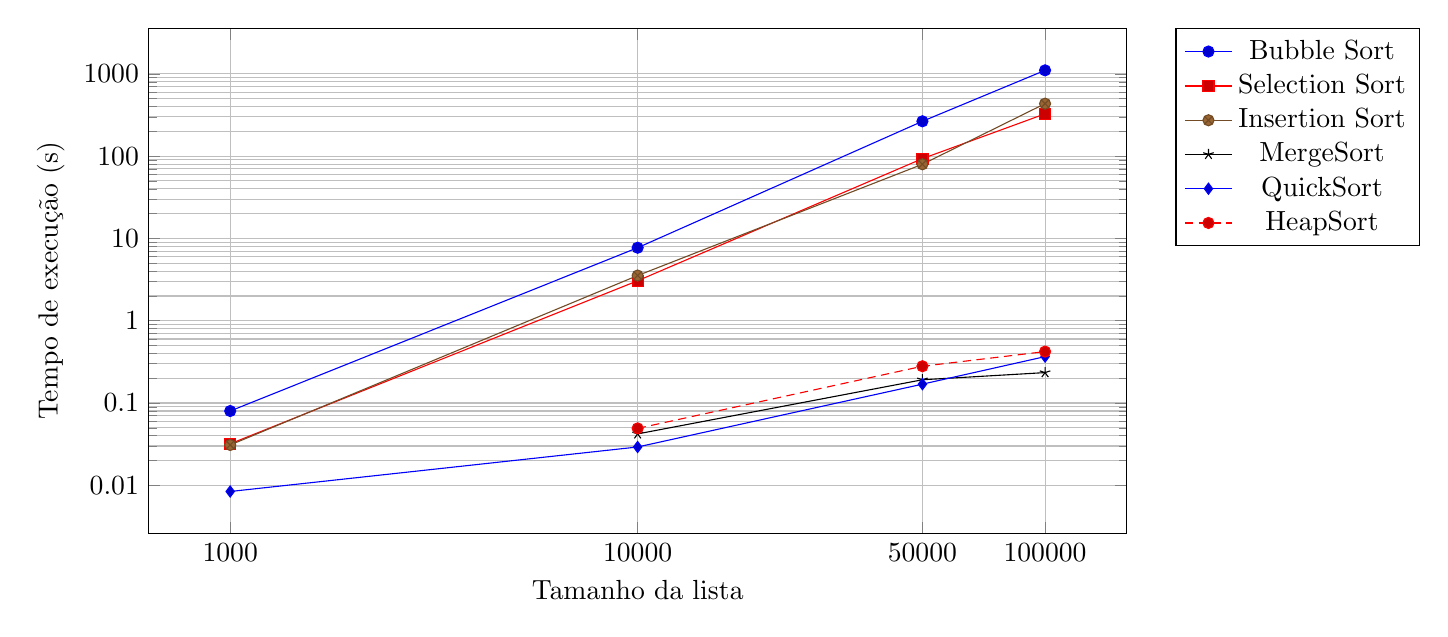
\begin{tikzpicture}
    \begin{loglogaxis}[
        width=14cm, height=8cm,
        xlabel={Tamanho da lista},
        ylabel={Tempo de execução (s)},
        legend style={at={(1.05,1)}, anchor=north west},
        grid=both,
        xtick={1000,10000,50000,100000},
        xticklabels={1000, 10000, 50000, 100000},
        ytick={0.01, 0.1, 1, 10, 100, 1000},
        yticklabels={0.01, 0.1, 1, 10, 100, 1000}
    ]

    % Bubble Sort
    \addplot coordinates {
        (1000, 0.079946)
        (10000, 7.714882)
        (50000, 265.328877)
        (100000, 1104.268497)
    };
    \addlegendentry{Bubble Sort}

    % Selection Sort
    \addplot coordinates {
        (1000, 0.031948)
        (10000, 3.060760)
        (50000, 93.325466)
        (100000, 327.016612)
    };
    \addlegendentry{Selection Sort}

    % Insertion Sort
    \addplot coordinates {
        (1000, 0.030918)
        (10000, 3.543290)
        (50000, 79.701274)
        (100000, 434.775822)
    };
    \addlegendentry{Insertion Sort}

    % MergeSort
    \addplot coordinates {
        (1000, 0.000000)
        (10000, 0.042150)
        (50000, 0.191727)
        (100000, 0.234253)
    };
    \addlegendentry{MergeSort}

    % QuickSort
    \addplot coordinates {
        (1000, 0.008410)
        (10000, 0.029226)
        (50000, 0.169494)
        (100000, 0.366376)
    };
    \addlegendentry{QuickSort}

    % HeapSort
    \addplot coordinates {
        (1000, 0.000000)
        (10000, 0.049189)
        (50000, 0.279829)
        (100000, 0.421897)
    };
    \addlegendentry{HeapSort}

    \end{loglogaxis}
    \end{tikzpicture}
    \caption{Comparação dos tempos de execução dos algoritmos de ordenação (distribuição aleatória)}
    \label{fig:sorting_algorithms}
\end{figure}

% Gráfico para distribuição Ordenada
\begin{figure}
    \centering
    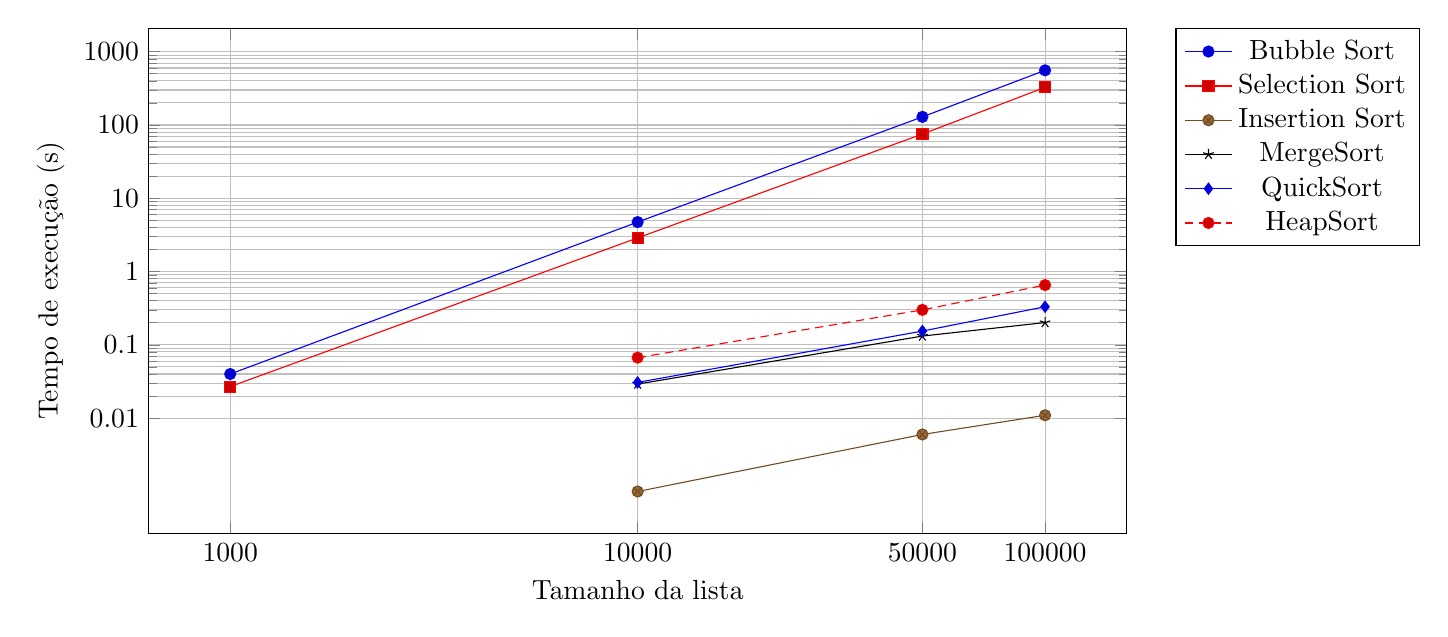
\begin{tikzpicture}
    \begin{loglogaxis}[
        width=14cm, height=8cm,
        xlabel={Tamanho da lista},
        ylabel={Tempo de execução (s)},
        legend style={at={(1.05,1)}, anchor=north west},
        grid=both,
        xtick={1000,10000,50000,100000},
        xticklabels={1000, 10000, 50000, 100000},
        ytick={0.01, 0.1, 1, 10, 100, 1000},
        yticklabels={0.01, 0.1, 1, 10, 100, 1000}
    ]

    % Bubble Sort
    \addplot coordinates {
        (1000, 0.039974)
        (10000, 4.732999)
        (50000, 129.089798)
        (100000, 556.851032)
    };
    \addlegendentry{Bubble Sort}

    % Selection Sort
    \addplot coordinates {
        (1000, 0.026921)
        (10000, 2.879377)
        (50000, 75.252023)
        (100000, 326.084314)
    };
    \addlegendentry{Selection Sort}

    % Insertion Sort
    \addplot coordinates {
        (1000, 0.000000)
        (10000, 0.000997)
        (50000, 0.005983)
        (100000, 0.010937)
    };
    \addlegendentry{Insertion Sort}

    % MergeSort
    \addplot coordinates {
        (1000, 0.000000)
        (10000, 0.029111)
        (50000, 0.131731)
        (100000, 0.201298)
    };
    \addlegendentry{MergeSort}

    % QuickSort
    \addplot coordinates {
        (1000, 0.000000)
        (10000, 0.030715)
        (50000, 0.154098)
        (100000, 0.331038)
    };
    \addlegendentry{QuickSort}

    % HeapSort
    \addplot coordinates {
        (1000, 0.000000)
        (10000, 0.066907)
        (50000, 0.299867)
        (100000, 0.653998)
    };
    \addlegendentry{HeapSort}

    \end{loglogaxis}
    \end{tikzpicture}
    \caption{Comparação dos tempos de execução dos algoritmos de ordenação (distribuição ordenada)}
    \label{fig:sorting_algorithms_ordered}
\end{figure}

% Gráfico para distribuição Inversamente Ordenada
\begin{figure}
    \centering
    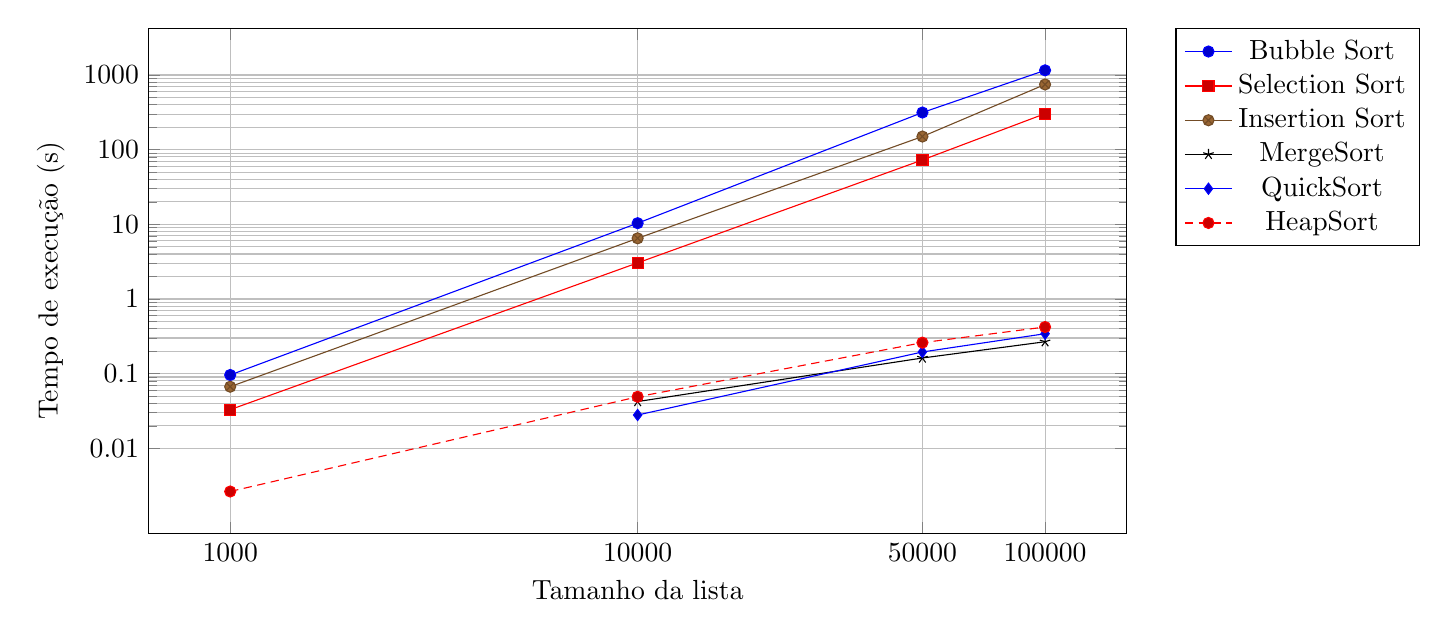
\begin{tikzpicture}
    \begin{loglogaxis}[
        width=14cm, height=8cm,
        xlabel={Tamanho da lista},
        ylabel={Tempo de execução (s)},
        legend style={at={(1.05,1)}, anchor=north west},
        grid=both,
        xtick={1000,10000,50000,100000},
        xticklabels={1000, 10000, 50000, 100000},
        ytick={0.01, 0.1, 1, 10, 100, 1000},
        yticklabels={0.01, 0.1, 1, 10, 100, 1000}
    ]

    % Bubble Sort
    \addplot coordinates {
        (1000, 0.095963)
        (10000, 10.361087)
        (50000, 314.585078)
        (100000, 1155.711274)
    };
    \addlegendentry{Bubble Sort}

    % Selection Sort
    \addplot coordinates {
        (1000, 0.032912)
        (10000, 3.046849)
        (50000, 72.830210)
        (100000, 303.780485)
    };
    \addlegendentry{Selection Sort}

    % Insertion Sort
    \addplot coordinates {
        (1000, 0.066811)
        (10000, 6.496479)
        (50000, 150.014955)
        (100000, 747.859663)
    };
    \addlegendentry{Insertion Sort}

    % MergeSort
    \addplot coordinates {
        (1000, 0.000000)
        (10000, 0.042281)
        (50000, 0.162003)
        (100000, 0.267392)
    };
    \addlegendentry{MergeSort}

    % QuickSort
    \addplot coordinates {
        (1000, 0.000000)
        (10000, 0.027901)
        (50000, 0.195123)
        (100000, 0.342594)
    };
    \addlegendentry{QuickSort}

    % HeapSort
    \addplot coordinates {
        (1000, 0.002637)
        (10000, 0.048995)
        (50000, 0.260106)
        (100000, 0.421161)
    };
    \addlegendentry{HeapSort}

    \end{loglogaxis}
    \end{tikzpicture}
    \caption{Comparação dos tempos de execução dos algoritmos de ordenação (distribuição inversamente ordenada)}
    \label{fig:sorting_algorithms_reverse}
\end{figure}


\begin{flushleft}
% Alinha a tabela à esquerda
\scriptsize% Reduz o tamanho da fonte da tabela

\begin{longtable}{|l|l|l|l|l|l|}
\hline
\textbf{Algoritmo} & \textbf{Tamanho} & \textbf{Distribuição} & \textbf{Tempo (s)} & \textbf{Comparações} & \textbf{Trocas} \\
\hline
\endfirsthead
\hline
\textbf{Algoritmo} & \textbf{Tamanho} & \textbf{Distribuição} & \textbf{Tempo (s)} & \textbf{Comparações} & \textbf{Trocas} \\
\hline
\endhead
\hline
\endfoot

\hline

\textbf{Bubble Sort} & 1000 & Ordered & 0.039974 & 499500 & 0 \\
\textbf{Selection Sort} & 1000 & Ordered & 0.026921 & 499500 & 0 \\
\textbf{Insertion Sort} & 1000 & Ordered & 0.000000 & 999 & 0 \\
\textbf{MergeSort} & 1000 & Ordered & 0.000000 & 4932 & 0 \\
\textbf{QuickSort} & 1000 & Ordered & 0.000000 & 10765 & 7016 \\
\textbf{HeapSort} & 1000 & Ordered & 0.000000 & 17583 & 9708 \\
\hline
\textbf{Bubble Sort} & 1000 & Reverse & 0.095963 & 499500 & 499500 \\
\textbf{Selection Sort} & 1000 & Reverse & 0.032912 & 499500 & 500 \\
\textbf{Insertion Sort} & 1000 & Reverse & 0.066811 & 500499 & 499500 \\
\textbf{MergeSort} & 1000 & Reverse & 0.000000 & 5044 & 5044 \\
\textbf{QuickSort} & 1000 & Reverse & 0.000000 & 9795 & 6294 \\
\textbf{HeapSort} & 1000 & Reverse & 0.002637 & 15965 & 8316 \\
\hline
\textbf{Bubble Sort} & 1000 & Random & 0.079946 & 499500 & 254209 \\
\textbf{Selection Sort} & 1000 & Random & 0.031948 & 499500 & 995 \\
\textbf{Insertion Sort} & 1000 & Random & 0.030918 & 248669 & 247670 \\
\textbf{MergeSort} & 1000 & Random & 0.000000 & 8677 & 4421 \\
\textbf{QuickSort} & 1000 & Random & 0.008410 & 10630 & 7134 \\
\textbf{HeapSort} & 1000 & Random & 0.000000 & 16848 & 9082 \\
\hline
\textbf{Bubble Sort} & 10000 & Ordered & 4.732999 & 49995000 & 0 \\
\textbf{Selection Sort} & 10000 & Ordered & 2.879377 & 49995000 & 0 \\
\textbf{Insertion Sort} & 10000 & Ordered & 0.000997 & 9999 & 0 \\
\textbf{MergeSort} & 10000 & Ordered & 0.029111 & 64608 & 0 \\
\textbf{QuickSort} & 10000 & Ordered & 0.030715 & 155057 & 85121 \\
\textbf{HeapSort} & 10000 & Ordered & 0.066907 & 244460 & 131956 \\
\hline
\textbf{Bubble Sort} & 10000 & Reverse & 10.361087 & 49995000 & 49995000 \\
\textbf{Selection Sort} & 10000 & Reverse & 3.046849 & 49995000 & 5000 \\
\textbf{Insertion Sort} & 10000 & Reverse & 6.496479 & 50004999 & 49995000 \\
\textbf{MergeSort} & 10000 & Reverse & 0.042281 & 69008 & 69008 \\
\textbf{QuickSort} & 10000 & Reverse & 0.027901 & 147613 & 82225 \\
\textbf{HeapSort} & 10000 & Reverse & 0.048995 & 226682 & 116696 \\
\hline
\textbf{Bubble Sort} & 10000 & Random & 7.714882 & 49995000 & 25186758 \\
\textbf{Selection Sort} & 10000 & Random & 3.060760 & 49995000 & 9952 \\
\textbf{Insertion Sort} & 10000 & Random & 3.543290 & 25247651 & 25237652 \\
\textbf{MergeSort} & 10000 & Random & 0.042150 & 120533 & 61231 \\
\textbf{QuickSort} & 10000 & Random & 0.029226 & 153586 & 92592 \\
\textbf{HeapSort} & 10000 & Random & 0.049189 & 235296 & 124159 \\
\hline
\textbf{Bubble Sort} & 50000 & Ordered & 129.089798 & 1249975000 & 0 \\
\textbf{Selection Sort} & 50000 & Ordered & 75.252023 & 1249975000 & 0 \\
\textbf{Insertion Sort} & 50000 & Ordered & 0.005983 & 49999 & 0 \\
\textbf{MergeSort} & 50000 & Ordered & 0.131731 & 382512 & 0 \\
\textbf{QuickSort} & 50000 & Ordered & 0.154098 & 918778 & 517246 \\
\textbf{HeapSort} & 50000 & Ordered & 0.299867 & 1455438 & 773304 \\
\hline
\textbf{Bubble Sort} & 50000 & Reverse & 314.585078 & 1249975000 & 1249975000 \\
\textbf{Selection Sort} & 50000 & Reverse & 72.830210 & 1249975000 & 25000 \\
\textbf{Insertion Sort} & 50000 & Reverse & 150.014955 & 1250024999 & 1249975000 \\
\textbf{MergeSort} & 50000 & Reverse & 0.162003 & 401952 & 401952 \\
\textbf{QuickSort} & 50000 & Reverse & 0.195123 & 926038 & 507124 \\
\textbf{HeapSort} & 50000 & Reverse & 0.260106 & 1366047 & 698892 \\
\hline
\textbf{Bubble Sort} & 50000 & Random & 265.328877 & 1249975000 & 628345568 \\
\textbf{Selection Sort} & 50000 & Random & 93.325466 & 1249975000 & 49989 \\
\textbf{Insertion Sort} & 50000 & Random & 79.701274 & 623335460 & 623285461 \\
\textbf{MergeSort} & 50000 & Random & 0.191727 & 718322 & 363440 \\
\textbf{QuickSort} & 50000 & Random & 0.169494 & 919639 & 526873 \\
\textbf{HeapSort} & 50000 & Random & 0.279829 & 1409966 & 737489 \\
\hline
\textbf{Bubble Sort} & 100000 & Ordered & 556.851032 & 4999950000 & 0 \\
\textbf{Selection Sort} & 100000 & Ordered & 326.084314 & 4999950000 & 0 \\
\textbf{Insertion Sort} & 100000 & Ordered & 0.010937 & 99999 & 0 \\
\textbf{MergeSort} & 100000 & Ordered & 0.201298 & 815024 & 0 \\
\textbf{QuickSort} & 100000 & Ordered & 0.331038 & 2011480 & 1157392 \\
\textbf{HeapSort} & 100000 & Ordered & 0.653998 & 3112517 & 1650854 \\
\hline
\textbf{Bubble Sort} & 100000 & Reverse & 1155.711274 & 4999950000 & 4999950000 \\
\textbf{Selection Sort} & 100000 & Reverse & 314.536680 & 4999950000 & 50000 \\
\textbf{Insertion Sort} & 100000 & Reverse & 648.021695 & 5000049999 & 4999950000 \\
\textbf{MergeSort} & 100000 & Reverse & 0.295214 & 835484 & 835484 \\
\textbf{QuickSort} & 100000 & Reverse & 0.349702 & 1865619 & 1074137 \\
\textbf{HeapSort} & 100000 & Reverse & 0.573763 & 2815541 & 1473448 \\
\hline
\textbf{Bubble Sort} & 100000 & Random & 1012.794162 & 4999950000 & 2420306761 \\
\textbf{Selection Sort} & 100000 & Random & 334.304135 & 4999950000 & 99977 \\
\textbf{Insertion Sort} & 100000 & Random & 296.111688 & 2499943406 & 2499443407 \\
\textbf{MergeSort} & 100000 & Random & 0.235746 & 1000662 & 500538 \\
\textbf{QuickSort} & 100000 & Random & 0.282716 & 2009520 & 1152444 \\
\textbf{HeapSort} & 100000 & Random & 0.525115 & 3105785 & 1614447 \\
\hline

\end{longtable}

\end{flushleft}



\section{Discussão}
\subsection{Análise dos resultados comparando com as expectativas teóricas.}
Os resultados obtidos para os algoritmos de ordenação \textit{Bubble Sort}, \textit{Selection Sort} e \textit{Insertion Sort} refletem claramente o comportamento teórico previsto, especialmente no que tange à complexidade computacional e à eficiência relativa para diferentes tipos de entrada.

O \textit{Bubble Sort}, conhecido por sua baixa eficiência em grandes volumes de dados, apresenta uma complexidade de \( O(n^2) \) tanto em termos de comparações quanto de trocas. Isso é evidente nos experimentos, onde o tempo de execução cresce exponencialmente conforme o tamanho da lista aumenta, especialmente para listas inversamente ordenadas. No caso de listas já ordenadas, o número de trocas é zero, como previsto, pois o algoritmo reconhece que a lista está ordenada. No entanto, ainda são realizadas \( n(n-1)/2 \) comparações, resultando em tempos de execução relativamente altos, mesmo neste cenário. Para listas inversamente ordenadas, tanto o número de comparações quanto o de trocas é máximo, refletindo o comportamento de pior caso do algoritmo. Com listas aleatórias, o desempenho do \textit{Bubble Sort} se situa entre os dois extremos, confirmando o comportamento teórico esperado.

O \textit{Selection Sort}, também com complexidade \( O(n^2) \), diferencia-se pelo número reduzido de trocas. Mesmo no melhor caso (lista ordenada), ele realiza \( n(n-1)/2 \) comparações, como evidenciado nos tempos de execução, mas o número de trocas é significativamente menor comparado ao \textit{Bubble Sort}, pois o \textit{Selection Sort} realiza no máximo \( n-1 \) trocas, independentemente da ordenação inicial. Para listas inversamente ordenadas e aleatórias, houve um aumento no número de trocas, mas ainda assim inferior ao \textit{Bubble Sort}, o que explica seu desempenho relativamente melhor nos experimentos.

O \textit{Insertion Sort}, por sua vez, confirma sua eficiência teórica em cenários onde a lista já está ordenada ou quase ordenada. No melhor caso (lista já ordenada), sua complexidade é linear, \( O(n) \), o que é observado no tempo de execução extremamente baixo e no pequeno número de comparações e trocas. No pior caso (lista inversamente ordenada), a complexidade é \( O(n^2) \), como mostrado nos resultados experimentais, com tempos de execução altos e um grande número de comparações e trocas. Para listas aleatórias, o desempenho do \textit{Insertion Sort} situa-se entre esses dois extremos, como esperado.

Assim, os resultados experimentais estão em plena conformidade com a teoria. Algoritmos como o \textit{Insertion Sort} são bastante eficientes para listas pequenas ou quase ordenadas, enquanto \textit{Bubble Sort} e \textit{Selection Sort} são prejudicados por sua complexidade quadrática. O \textit{Bubble Sort} é particularmente ineficiente em listas inversamente ordenadas, enquanto o \textit{Selection Sort} mantém um número constante de comparações, independentemente da ordem dos dados. Para grandes volumes de dados desordenados, todos os três algoritmos tornam-se impraticáveis em termos de tempo de execução, conforme o esperado teoricamente.

Os resultados obtidos para os algoritmos \textit{MergeSort}, \textit{QuickSort} e \textit{HeapSort} em diferentes tamanhos de entrada e distribuições confirmam as expectativas teóricas quanto ao desempenho e comportamento de cada algoritmo.

O \textit{MergeSort}, com complexidade \( O(n \log n) \), apresentou comportamento consistente tanto em termos de tempo de execução quanto em número de comparações e trocas. Para listas ordenadas, o \textit{MergeSort} realiza um número fixo de comparações \( \approx n \log n \), sem a necessidade de trocas. 

Para listas de tamanho 100.000 e ordenadas, o \textit{MergeSort} executou em \textbf{0.201298s} com \textbf{815024} comparações e \textbf{0} trocas. Já para listas inversamente ordenadas e aleatórias, o número de comparações e trocas foi maior, mas o tempo de execução continuou competitivo.

O \textit{QuickSort} apresentou resultados condizentes com sua complexidade \( O(n^2) \) no pior caso e \( O(n \log n) \) no melhor caso. Em listas ordenadas, o \textit{QuickSort} sofre com o número elevado de comparações e trocas. Em uma lista de 100.000 elementos ordenados, ele realizou \textbf{2011480 comparações} e \textbf{1157392 trocas}, com tempo de \textbf{0.331038s}. Para listas inversamente ordenadas, o comportamento foi semelhante, enquanto para listas aleatórias, o algoritmo foi mais eficiente, apesar de realizar mais trocas.

O \textit{HeapSort} foi o mais lento entre os três, com complexidade \( O(n \log n) \), mas com maior número de comparações e trocas. Para listas de 100.000 elementos ordenados, ele realizou \textbf{3112517 comparações} e \textbf{1650854 trocas}, com tempo de \textbf{0.653998s}. Esse comportamento se repetiu nas listas inversamente ordenadas e aleatórias, com números significativamente altos de comparações e trocas.

Em termos de eficiência, o \textit{MergeSort} foi o algoritmo mais estável e previsível em todos os cenários. O \textit{QuickSort} mostrou eficiência em listas aleatórias, mas apresentou um desempenho ruim para listas ordenadas e inversamente ordenadas. O \textit{HeapSort}, por fim, foi o menos eficiente em termos de tempo e número de operações, sendo penalizado pelo grande número de trocas.

\subsection{Considerações sobre a facilidade de implementação, uso de memória e estabilidade dos algoritmos.}

A escolha adequada de um algoritmo de ordenação deve levar em consideração fatores como a facilidade de implementação, o uso de memória e a estabilidade. Cada um desses aspectos é analisado a seguir para os algoritmos abordados neste trabalho.

\subsubsection{Facilidade de Implementação}
A facilidade de implementação dos algoritmos varia conforme sua complexidade. Algoritmos simples, como o \textit{Bubble Sort}, \textit{Selection Sort} e \textit{Insertion Sort}, são reconhecidos por suas estruturas diretas e intuitivas, sendo amplamente utilizados para fins educacionais devido à facilidade de compreensão. Esses algoritmos envolvem loops simples e poucas variáveis auxiliares, facilitando sua codificação.

Por outro lado, algoritmos como o \textit{MergeSort}, \textit{QuickSort} e \textit{HeapSort} são mais complexos de implementar. O \textit{MergeSort}, por exemplo, requer uma função auxiliar para mesclar sublistas e o uso de recursão, enquanto o \textit{QuickSort} exige uma escolha cuidadosa do pivô e uma divisão eficiente do array, fatores que impactam diretamente seu desempenho. O \textit{HeapSort}, por sua vez, requer o uso de uma estrutura de dados como o heap binário, demandando maior entendimento do programador.

\subsubsection{Uso de Memória}
O uso de memória também varia consideravelmente entre os algoritmos:

\begin{itemize}
    \item O \textit{Bubble Sort}, \textit{Selection Sort} e \textit{Insertion Sort} são algoritmos \textit{in-place}, isto é, operam diretamente no array de entrada, sem necessidade de espaço adicional significativo, com complexidade de espaço \( O(1) \). 
    \item O \textit{MergeSort}, por outro lado, requer espaço adicional proporcional ao tamanho do array devido à criação de cópias temporárias durante o processo de divisão e mesclagem das sublistas. Assim, sua complexidade de espaço é \( O(n) \), podendo ser limitante em aplicações com grandes volumes de dados.
    \item O \textit{QuickSort} é geralmente \textit{in-place}, com uso de memória \( O(\log n) \) no melhor caso devido à recursão. No entanto, no pior caso, a profundidade da pilha de recursão pode alcançar \( O(n) \).
    \item O \textit{HeapSort} também é \textit{in-place}, com complexidade de espaço \( O(1) \), utilizando o próprio array para construir a estrutura heap, o que torna seu uso de memória eficiente.
\end{itemize}

\subsubsection{Estabilidade}
A estabilidade dos algoritmos indica se a ordem relativa dos elementos com chaves iguais é preservada após a ordenação. Este aspecto é essencial em algumas aplicações, especialmente onde há múltiplos critérios de ordenação.

\begin{itemize}
    \item O \textit{Bubble Sort} e o \textit{Insertion Sort} são algoritmos estáveis, pois trocam elementos apenas quando necessário, mantendo a ordem relativa entre elementos iguais.
    \item O \textit{Selection Sort}, \textit{QuickSort} e \textit{HeapSort} não são estáveis. O \textit{Selection Sort} realiza trocas diretas entre elementos de posições distantes, enquanto o \textit{QuickSort}, dependendo da implementação, pode trocar o pivô com outros elementos, prejudicando a estabilidade. O \textit{HeapSort} organiza o array em uma estrutura heap, o que elimina a ordem relativa entre elementos iguais.
    \item O \textit{MergeSort} é um algoritmo estável, pois suas operações de divisão e mesclagem preservam a ordem relativa dos elementos. Isso o torna ideal em aplicações onde a estabilidade é um requisito.
\end{itemize}

\subsection{Discussão sobre as limitações do trabalho e sugestões para estudos futuros.}

Este trabalho realizou uma análise dos algoritmos de ordenação \textit{Bubble Sort}, \textit{Selection Sort}, \textit{Insertion Sort}, \textit{MergeSort}, \textit{QuickSort} e \textit{HeapSort}, considerando aspectos de desempenho e complexidade. No entanto, algumas limitações devem ser destacadas para contextualizar os resultados obtidos e guiar pesquisas futuras.

\subsubsection{Limitações do Trabalho}
\begin{itemize}
    
    \item \textbf{Ambiente de testes controlado}: Os experimentos foram realizados em um ambiente controlado, sem variações de hardware e sistema operacional, o que limita a generalização dos resultados para outros ambientes de execução. Desempenho e eficiência podem variar significativamente em diferentes arquiteturas e condições de operação.


\end{itemize}

\subsubsection{Sugestões para Estudos Futuros}
Algumas direções são sugeridas para estudos futuros:

\begin{itemize}
    \item \textbf{Incluir algoritmos modernos e híbridos}: Estudos futuros podem ampliar a análise ao incluir algoritmos de ordenação híbridos, como o \textit{TimSort}, que combina \textit{Merge Sort} e \textit{Insertion Sort}, e outros algoritmos não comparativos, como o \textit{Radix Sort}, que tem um desempenho muito melhor para dados inteiros.
    
    \item \textbf{Avaliação em diferentes ambientes de hardware}: Realizar experimentos em diversas plataformas, incluindo processadores de diferentes arquiteturas, dispositivos móveis e ambientes de nuvem, ajudaria a entender como os algoritmos se comportam em diferentes contextos de execução, além de analisar o impacto do paralelismo em algoritmos que podem ser otimizados para multi-threading.


    
\end{itemize}

\section{Conclusão}
\subsection{Síntese dos principais achados do trabalho.}
Este trabalho realizou uma análise detalhada dos algoritmos de ordenação \textit{Bubble Sort}, \textit{Selection Sort}, \textit{Insertion Sort}, \textit{MergeSort}, \textit{QuickSort} e \textit{HeapSort}, com foco em suas características de desempenho, complexidade computacional e uso de memória. Abaixo, resumem-se os principais achados:

\begin{itemize}
    \item \textbf{Desempenho em relação à complexidade}: Os experimentos confirmaram a complexidade teórica esperada para cada algoritmo. 

    \item \textbf{Eficiência dos algoritmos \( O(n \log n) \)}: Os algoritmos \textit{MergeSort}, \textit{QuickSort} e \textit{HeapSort}, que possuem complexidade \( O(n \log n) \), demonstraram um desempenho superior para grandes volumes de dados.

    \item \textbf{Estabilidade}: Dentre os algoritmos analisados, apenas o \textit{Bubble Sort}, \textit{Insertion Sort} e \textit{MergeSort} são algoritmos estáveis, preservando a ordem relativa dos elementos iguais. 

    \item \textbf{Uso de memória}: O estudo demonstrou que o uso de memória varia conforme o algoritmo. \textit{Bubble Sort}, \textit{Selection Sort}, \textit{Insertion Sort} e \textit{HeapSort} são algoritmos \textit{in-place}, que operam com \( O(1) \) de complexidade de espaço adicional, o que os torna eficientes em termos de uso de memória. \textit{MergeSort}, no entanto, requer \( O(n) \) de memória adicional para a criação de sublistas, enquanto o \textit{QuickSort} possui uma complexidade de espaço \( O(\log n) \) em média, mas pode atingir \( O(n) \) no pior caso, devido à recursão.

\end{itemize}

\subsection{Recomendações sobre o uso de cada algoritmo em diferentes situações.}
Algoritmos \( O(n^2) \), como o Bubble Sort, Selection Sort e Insertion Sort, tiveram uma performance significativamente pior para listas grandes, especialmente no caso de dados reversos e aleatórios.

Algoritmos \( O(n \log n) \), como MergeSort, QuickSort e HeapSort, apresentaram um desempenho superior, com tempos de execução mais rápidos e um número menor de comparações e trocas.

Em geral, para listas pequenas, os algoritmos \( O(n^2) \) ainda podem ser aceitáveis, mas para listas maiores, os algoritmos \( O(n \log n) \) são muito mais eficientes.


\section{Referências}
\subsection{Listagem das fontes utilizadas para a revisão teórica e fundamentação do trabalho.}

\begin{itemize}
    \item CORMEN, T. H.; LEISERSON, C. E.; RIVEST, R. L.; STEIN, C. \textit{Introduction to Algorithms}. 3ª edição. MIT Press, 2009.
    \item SEDGEWICK, R.; WAYNE, K. \textit{Algorithms}. 4ª edição. Addison-Wesley, 2011.
    \item WEISS, M. A. \textit{Data Structures and Algorithm Analysis in C++}. 4ª edição. Pearson, 2014.
    \item KNUTH, D. E. \textit{The Art of Computer Programming, Volume 3: Sorting and Searching}. 2ª edição. Addison-Wesley, 1998.
    \item SAHNI, S. \textit{Data Structures, Algorithms, and Applications in C++}. 2ª edição. McGraw-Hill, 2005.
    \item GOODRICH, M. T.; TAMASSIA, R. \textit{Algorithm Design: Foundations, Analysis, and Internet Examples}. 2ª edição. John Wiley \& Sons, 2006.
    \item HOARE, C. A. R. "Quicksort." \textit{The Computer Journal}, Volume 5, Issue 1, 1962.
    \item WILLIAMS, J. W. J. "Algorithm 232: Heapsort." 
    \item Slides Professor Warley Gramacho\\
    \textit{Communications of the ACM}, Volume 7, Issue 6, 1964.
\end{itemize}

\end{document}
